\section{Geometri}
Pada dasarnya geometri di olimpiade matematika SMA "hanya" tentang lingkaran dan segitiga dua dimensi (Soal bangun tiga dimensi hampir ngga pernah dikeluarin untuk lomba tingkat SMA).
\subsection{Garis, Segmen Garis, Sinar (Bukan Vektor!)}
    Perlu ditekankan bahwa \textbf{garis tidak sama dengan ruas garis}. Garis panjangnya tak hingga, sedangkan ruas garis atau segmen garis panjangnya terbatas. Gambar di bawah terdiri dari \textbf{garis AB, segmen garis CD, sinar EF}.
\begin{center}
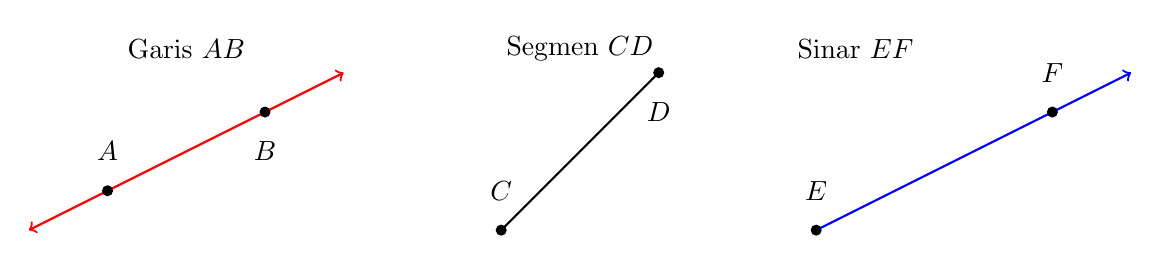
\begin{tikzpicture}
    % Draw a line
    \draw[red, thick, <->] (-4,-1) -- (0,1);
    \node at (-2,1.3) {Garis $AB$};
    \fill (-3,-0.5) circle (2pt);
    \fill (-1,0.5) circle (2pt);
    \node at (-3,-0) {$A$};
    \node at (-1,0) {$B$};

    % Draw a segment
    \draw[thick] (2,-1) -- (4,1);
    \node at (3,1.3) {Segmen $CD$};
    \fill (2,-1) circle (2pt);
    \fill (4,1) circle (2pt);
    \node at (2,-0.5) {$C$};
    \node at (4,0.5) {$D$};

    % Draw a ray
    \draw[blue, thick, ->] (6,-1) -- (10,1);
    \node at (6.5,1.3) {Sinar $EF$};
    \fill (6,-1) circle (2pt);
    \fill (9,0.5) circle (2pt);
    \node at (6,-0.5) {$E$};
    \node at (9,1) {$F$};
\end{tikzpicture}
\end{center}
\subsection{Lingkaran}

\begin{center}
\begin{tikzpicture}
\coordinate (O) at (0,0);
\coordinate (B) at (0:2cm);
\coordinate (A) at (210:2cm);
\coordinate (D) at (180:2cm);
\coordinate (C) at (130:2cm);
\coordinate (E) at (-20:2cm);

\draw (O) circle (2cm);

\draw (A) -- (B) -- (C) -- (D) -- cycle;
\draw (A) -- (E) -- (C);
\draw[red] (A) -- (C);

\tkzDefPointBy[projection=onto A--C](O) \tkzGetPoint{F}
\draw[orange] (O) -- (F);
\draw[blue] (C) -- (O) -- (A);

\node[right] at (B) {$B$};
\node[below left] at (A) {$A$};
\node[left] at (D) {$D$};
\node[above left] at (C) {$C$};
\node[below right] at (E) {$E$};
\node[right] at (O) {$O$};
\node[above right] at (F) {$F$};
\end{tikzpicture}
\end{center}

    
Misalkan $O$ pusat lingkaran $\Gamma$ dan $A,B,C,D,E$ adalah sembarang titik pada lingkaran $\Gamma$ seperti pada gambar.
\begin{enumerate}
    \item $CO=OA$ adalah jari-jari dengan $\angle ACO = \angle OAC$.
    \item Misalkan titik $F$ adalah titik tengah tali busur $CA$, maka $OF \perp CA$ atau $OF$ tegak lurus dengan $CA$, dengan kata lain, $F$ adalah proyeksi titik $O$ ke $CA$
    \item (Sudut keliling-sudut pusat) Untuk$\angle COA = 2\angle CBA$.
    \item (sudut keliling) $\angle CBA = \angle CEA$.
    \item $ABCD$ adalah segiempat tali busur atau segiempat siklis  atau $A,B,C,D$ terletak di lingkaran (seperti pada gambar) jika dan hanya jika $\angle CBA + \angle ADC = 180^\circ$ atau $\angle ABD = \angle ACD$.
\end{enumerate}
\subsection{Latihan Soal Lingkaran}
\begin{enumerate}
    \item Pada segiempat $WXYZ$ dengan diagonal yang saling tegak lurus diketahui bahwa $\angle WZX = 30^\circ, \angle XWY = 40^\circ,$ and $\angle WYZ = 50^\circ$. Hitunglah besar $\angle X$ dan $\angle Z$.
    \begin{center}
        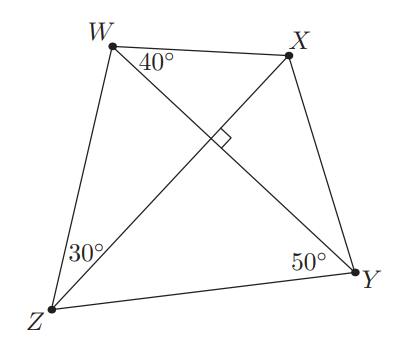
\includegraphics[width=0.25\textwidth]{assets/evanquad.PNG}
    \end{center}
		
    \item (OSK 2013) Diberikan segitiga lancip $ABC$ dengan $O$ sebagai pusat lingkaran luarnya. Misalkan $M$ dan $N$ berturut - turut pertengahan $OA$ dan $BC$. Jika $\angle ABC = 4\angle OMN$ dan $\angle ACB = 6\angle OMN$, maka besarnya $\angle OMN$ sama dengan \dots

    \item 	Pada gambar di bawah, diketahui titik A $\ne$ B pada lingkaran berdiameter $MN$ dan berpusat di $C$. $P$ adalah titik pada segmen $CN$ dimana $\angle CAP = \angle CBP = 10 ^\circ$. Jika $\angle ACM = 40^\circ$, maka $\angle BCN = \dots^\circ$	
    \begin{center}
         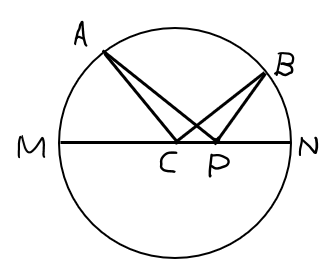
\includegraphics[width=0.25\textwidth]{assets/soalLingkaran1.PNG}
    \end{center}

    \item (OSK 2011,2012,2013,2018) Diberikan segitiga $ABC$ dan lingkaran $\Gamma$ yang berdiameter $AB$. Lingkaran $\Gamma$ memotong sisi $AC$ dan $BC$ berturut-turut di titik $D$ dan $E$. Jika $AD = \frac13 AC, BE =\frac14 BC$ dan $AB = 30$, maka luas segitiga $ABC$ adalah \dots

    \item (OSK 2015) Diberikan segitiga $ABC$ dengan sudut $\angle ABC = 90^\circ$. Lingkaran $L_1$ dengan $AB$ sebagai diameter sedangkan lingkaran $L_2$ dengan $BC$ sebagai diameternya. Kedua lingkaran $L_1$ dan $L_2$ berpotongan di $B$ dan $P$. Jika $AB = 5$, $BC = 12$ dan $BP = x$ maka nilai dari $\frac{240}{x}$ adalah \ldots
\end{enumerate}
\subsection{Segitiga}
Pada segitiga $ABC$ seperti gambar berikut:
\begin{center}
\begin{tikzpicture}
    % Define the coordinates of the vertices
    \coordinate (A) at (0,0);
    \coordinate (B) at (8,0);
    \coordinate (C) at (1.5,4);
    
    % Draw the triangle
    \draw (A) -- (B) -- (C) -- cycle;
    
    % circumcircle
    \tkzCircumCenter(A,B,C)\tkzGetPoint{O}
    \tkzDrawPoint(O)
    \tkzDrawCircle(O,A)
    
    % incircle
    \tkzDefCircle[in](A,B,C)\tkzGetPoint{I}\tkzGetLength{rIN}
    \tkzDrawPoint(I)
    \tkzDrawCircle[R](I,\rIN pt)
    
    % angle bisector
    \tkzDrawBisector[blue](B,A,C)\tkzGetPoint{E}
    \tkzDrawCircle[R](E,1 pt)
    
    %altitude
    \tkzDefPointBy[projection=onto B--C](A) \tkzGetPoint{D}
    \tkzDefPointBy[projection=onto B--A](C) \tkzGetPoint{C1}
    \tkzInterLL(A,D)(C,C1) \tkzGetPoint{H}
    \tkzDrawPoints(H) \tkzLabelPoints[below right](H)
    \tkzDrawSegment[red](A,D)
    \tkzDrawSegment[red](C,C1)

    %garis sumbu
    \tkzDefPointBy[projection=onto B--C](O) \tkzGetPoint{M}
    \tkzDefPointBy[homothety=center O ratio 3.2](M) \tkzGetPoint{M1}
    \tkzDefPointBy[homothety=center O ratio -3.2](M) \tkzGetPoint{M2}
    \tkzDrawSegment(M1,M2)
    \tkzDefPointBy[projection=onto B--A](O) \tkzGetPoint{M3}

    %centroid
    \tkzDrawSegment[green](A,M)
    \tkzDrawSegment[green](C,M3)
    \tkzInterLL(A,M)(C,M3) \tkzGetPoint{G}
    \tkzDrawPoints(G) \tkzLabelPoints[below right](G)
    
    % Label the vertices
    \node[below left] at (A) {$A$};
    \node[below right] at (B) {$B$};
    \node[above] at (C) {$C$};
    \node[below right] at (I) {$I$};
    \node[right] at (O) {$O$};
    \node[above right] at (E) {$E$};
    \node[above] at (D) {$D$};
    \node[right] at (M) {$M$};
\end{tikzpicture}
\end{center}
\begin{enumerate}
    \item Garis bagi $AE$ yaitu garis yang membagi dua sudut $A$ sama besar sehingga $\angle BAE = \angle EAC$. 
    \item Garis berat $AM$ dengan $M$ adalah titik tengah $BC$.
    \item Garis tinggi $AD$ adalah garis yang tegak lurus dengan $BC$. $D$ biasa disebut dengan proyeksi $A$ ke $BC$.
    \item Garis $OM$ adalah salah satu garis sumbu segitiga $ABC$, yaitu garis yang melewati titik tengah sisi segitiga dan tegak lurus dengan sisi itu.
    \item Pertemuan atau perpotongan ketiga garis tinggi segitiga $ABC$ adalah titik tinggi, dalam gambar ini adalah $H$ (orthocenter).
    \item Pertemuan atau perpotongan ketiga garis bagi segitiga $ABC$ adalah titik bagi atau titik pusat lingkaran dalam (incircle) segitiga $ABC$ dalam gambar ini adalah $I$ (incenter).
    \item Pertemuan atau perpotongan ketiga garis berat segitiga $ABC$ adalah titik berat (centroid).
    \item Pertemuan atau perpotongan ketiga garis sumbu segitiga $ABC$ adalah titik pusat lingkaran luar (circumcircle) segitiga $ABC$ yang dalam gambar ini adalah $O$ (circumcenter).
    \item Berlaku \textbf{ketaksamaan segitiga} yaitu $AB+BC>CA$, $BC+CA>AB$, dan $CA+AB>BC$. Selain itu juga berlaku $|AB-BC|<CA$, $|BC-CA|<AB$, dan $|CA-AB|<BC$.
\end{enumerate}
\subsection{Kesebangunan Segitiga}
\begin{center}
\begin{tikzpicture}
  % First triangle
  \coordinate (A) at (0,0);
  \coordinate (B) at (3,0);
  \coordinate (C) at (2,2);
  \draw (A) -- (B) -- (C) -- cycle;

  % Second triangle
  \coordinate (D) at (6,0);
  \coordinate (E) at (12,0);
  \coordinate (F) at (8,4);
  \draw (D) -- (E) -- (F) -- cycle;

  % Labeling the vertices
  \node[below] at (A) {$A$};
  \node[below] at (B) {$B$};
  \node[above] at (C) {$C$};
  \node[below] at (D) {$D$};
  \node[below] at (E) {$E$};
  \node[above] at (F) {$F$};

  \draw pic[draw=green!30,fill=green!30,angle radius=0.5cm] {angle=A--C--B};
  \draw pic[draw=green!30,fill=green!30,angle radius=0.5cm] {angle=D--F--E};
  \draw pic[draw=red!30,fill=red!30,angle radius=0.5cm] {angle=B--A--C};
  \draw pic[draw=red!30,fill=red!30,angle radius=0.5cm] {angle=F--E--D};
  \draw pic[draw=blue!30,fill=blue!30,angle radius=0.5cm] {angle=C--B--A};
  \draw pic[draw=blue!30,fill=blue!30,angle radius=0.5cm] {angle=E--D--F};
\end{tikzpicture}
\end{center}



Segitiga $ABC$ dan $DEF$ sebangun atau $ABC \sim DEF$ jika dan hanya jika minimal salah satu syarat ini terpenuhi:
\begin{enumerate}
    \item $\angle ABC = \angle DEF$ dan $\angle BAC = \angle EDF$.
    \item $\dfrac{AB}{DE} = \dfrac{BC}{EF} = \dfrac{CA}{FD}$.
    \item $\dfrac{AB}{DE} = \dfrac{BC}{EF}$ dan $\angle ABC = \angle DEF$ (sudut yang diapit dua sisi yang diperbandingkan nilainya sama)
\end{enumerate}

\subsection{Kekongruenan Segitiga}
\begin{center}
\begin{tikzpicture}
  % First triangle
  \coordinate (A) at (0,0);
  \coordinate (B) at (3,0);
  \coordinate (C) at (2,2);
  \draw (A) -- (B) -- (C) -- cycle;

  % Second triangle
  \coordinate (D) at (6,0);
  \coordinate (E) at (9,0);
  \coordinate (F) at (7,2);
  \draw (D) -- (E) -- (F) -- cycle;

  % Labeling the vertices
  \node[below] at (A) {$A$};
  \node[below] at (B) {$B$};
  \node[above] at (C) {$C$};
  \node[below] at (D) {$D$};
  \node[below] at (E) {$E$};
  \node[above] at (F) {$F$};

  \draw pic[draw=green!30,fill=green!30,angle radius=0.5cm] {angle=A--C--B};
  \draw pic[draw=green!30,fill=green!30,angle radius=0.5cm] {angle=D--F--E};
  \draw pic[draw=red!30,fill=red!30,angle radius=0.5cm] {angle=B--A--C};
  \draw pic[draw=red!30,fill=red!30,angle radius=0.5cm] {angle=F--E--D};
  \draw pic[draw=blue!30,fill=blue!30,angle radius=0.5cm] {angle=C--B--A};
  \draw pic[draw=blue!30,fill=blue!30,angle radius=0.5cm] {angle=E--D--F};

    \tkzMarkSegment[pos=.5,mark=|](C,B)
    \tkzMarkSegment[pos=.5,mark=|](D,F)
    \tkzMarkSegment[pos=.5,mark=||](C,A)
    \tkzMarkSegment[pos=.5,mark=||](E,F)
    \tkzMarkSegment[pos=.5,mark=|||](B,A)
    \tkzMarkSegment[pos=.5,mark=|||](E,D)
\end{tikzpicture}
\end{center}

Sedangkan $ABC$ dan $DEF$ dikatakan kongruen atau $\triangle ABC \cong \triangle DEF$ jika dan hanya jika $AB=DE, BC=EF, CA=FD$ atau dengan kata lain kedua segitiga tersebut sebangun dan ada salah satu sisi dari kedua segitiga tersebut yang panjangnya sama. Simpelnya kongruen = sama persis.


\subsection{Teorema Pythagoras}
Salah satu teorema paling terkenal di kalangan awam (atau setidaknya di pop culture). Diberikan segitiga $ABC$ dengan sudut $C$ siku-siku. Jika panjang sisi $AB=c$, $BC=a$, dan $CA=b$, maka berlaku
\begin{align*}
    a^2+b^2=c^2
\end{align*}
\begin{center}
    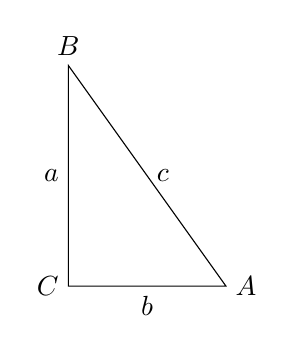
\begin{tikzpicture}
    % titik-titik segitiga
    \coordinate[label=left:$C$]  (C) at (-1.5cm,-1.cm);
    \coordinate[label=above:$B$] (B) at (-1.5cm,1.8cm);
    \coordinate[label=right:$A$] (A) at (0.5cm,-1.cm);
    
    % pembuatan segitiga
    \draw (A) -- node[right]{$c$} (B)  -- node[left]{$a$} (C) -- node[below]{$b$} cycle;
    \end{tikzpicture}
\end{center}
\subsection{Latihan Soal Segitiga }
\begin{enumerate}    
    \item Garis berat $AD$ pada segitiga $ABC$ memotong garis berat $CF$ di titik $P$, serta perpanjangan $BP$ memotong $AC$ di $E$. Jika diketahui segitiga $ABC$ lancip dan $AB=6$, maka panjang $DE$ adalah \dots

    \item (OSK 2011,2012,2013,2018) Diberikan segitiga $ABC$ dan lingkaran $\Gamma$ yang berdiameter $AB$. Lingkaran $\Gamma$ memotong sisi $AC$ dan $BC$ berturut-turut di titik $D$ dan $E$. Jika $AD = \frac13 AC, BE =\frac14 BC$ dan $AB = 30$, maka luas segitiga $ABC$ adalah \dots
		
    \item Diberikan segitiga $ABC$ dengan $D$ titik tengah $AC$, $E$ titik tengah $BD$, dan $H$ merupakan pencerminan $A$ terhadap $E$. Jika $F$ merupakan perpotongan antara $AH$ dengan $BC$, maka nilai $\dfrac{AF}{FH}$ sama dengan \dots
		 
    \item Diberikan segitiga $ABC$ dengan panjang sisi $BC = 20$, $CA = 24$, dan $AB=12$. Titik $D$ pada segmen $BC$ dengan $BD = 5$. Lingkaran luar dari segitiga $ABD$ memotong $CA$ di $E$. Hitunglah nilai $2 \times DE$.

    \item (OSK 2015) Diberikan trapesium $ABCD$ dengan $AB$ sejajar $DC$ dan $AB = 84$ serta $DC = 25$. Jika trapesium $ABCD$ memiliki lingkaran dalam yang menyinggung keempat sisinya, keliling trapesium $ABCD$ adalah \ldots

    \item (OSK 2022) Diberikan segitiga siku-siku $ABC$. Jika luas dari segitiga $ABC$ adalah 112. Misalkan $R$ adalah panjang jari-jari lingkaran luar segitiga $ABC$ dan $r$ adalah panjang jari-jari lingkaran dalam segitiga $ABC$. Diketahui juga $R + r = 16$. Panjang sisi miring dari segitiga $ABC$ adalah \ldots
\end{enumerate}
\subsection{Latihan Soal Pythagoras}
\begin{enumerate}
    \item (OSK SMP 2016) Diketahui $ABCD$ dan $CEGH$ adalah dua persegipanjang kongruen dengan panjang $17$ cm, dan lebar $8$ cm. Titik $E$ berada di sisi $AB$ dan $D$ berada di sisi $GH$. Titik $F$ adalah titik potong sisi $AD$ dan $EG$. Luas segiempat $EFDC$ adalah .... $cm^2$.

    \item Misalkan $ABC$ adalah segitiga lancip. Titik $D$, $E$, dan $F$ terletak pada sisi $BC$, $CA$, dan $AB$, berturut-turut, sedemikian sehingga $AD$, $BE$, dan $CF$ adalah garis tinggi segitiga $ABC$. Titik $H$ adalah titik tinggi segitiga $ABC$. Jika $DE = 8$, $DF = 15$, dan $EF = 17$, tentukan panjang $AH$.

    \item (OSK 2015) Diberikan segitiga $ABC$ dengan sudut $\angle ABC = 90^\circ$. Lingkaran $L_1$ dengan $AB$ sebagai diameter sedangkan lingkaran $L_2$ dengan $BC$ sebagai diameternya. Kedua lingkaran $L_1$ dan $L_2$ berpotongan di $B$ dan $P$. Jika $AB = 5$, $BC = 12$ dan $BP = x$ maka nilai dari $\frac{240}{x}$ adalah \ldots

    \item (OSK 2022) Diberikan segitiga $ABC$ siku-siku di B. Titik $D$ berada pada sisi $AB$ dan titik $E$ berada pada sisi $AC$. Diketahui $DE$ sejajar $BC$. Jika $AD = 21$, $DB = 3$, dan $BC = 32$, maka panjang $AE$ adalah \dots

\end{enumerate}
\subsection{Power of a point}
\begin{figure}[h]
  \begin{asy}
    unitsize(1.5cm);
    pair O, A, B, C, D, E, P;
    O = (0,0);
    P = (4,1);
    E = (0,1);
    A = dir(50);
    C = dir(-30);
    circle o = circumcircle(A,E,C);
    draw(o);
    pair B1[] = intersectionpoints(line(A,P), o);
    pair D1[] = intersectionpoints(line(C,P), o);
    B = B1[0];
    D = D1[0];
    draw(A--B);
    draw(C--D);
    draw(P--A);
    draw(P--D);
    draw(P--E, red);
    draw(P--O, blue+dotted);
    label("$O$",O,SW);
    label("$A$",A,E);
    label("$B$",B,N);
    label("$C$",C,SE);
    label("$D$",D,SW);
    label("$P$",P,NE);
    label("$E$",E,N);
    \end{asy}
    \begin{asy}
    unitsize(1.5cm);
    pair O, A, B, C, D, P;
    O = (0,0);
    A = dir(50);
    C = dir(130);
    D = dir(-30);
    B = dir(-110);
    P = extension(A,B,C,D);
    draw(circumcircle(A,B,C));
    draw(A--B);
    draw(C--D);
    draw(A--C--B--D--cycle);
    draw(O--P, dotted);
    label("$O$",O,SW);
    label("$A$",A,E);
    label("$B$",B,SW);
    label("$C$",C,NW);
    label("$D$",D,SE);
    label("$P$",P,E);
    \end{asy}
\end{figure}
Diberikan lingkaran $\Gamma$ dan titik $P$ yang terletak di dalam atau di luar lingkaran $\Gamma$. Maka definisikan kuasa atau power dari $P$ terhadap lingkaran $\Gamma$ sebagai
$$Pow_\Gamma (P) = |OP^2-r^2|$$
dimana $O$ adalah pusat dari $\Gamma$ dan $r$ adalah jari-jari lingkaran $\Gamma$.

Jika $A,B,C,D$ berada di $\Gamma$, serta $AB$ dan $CD$ berpotongan di $P$, maka $$Pow_\Gamma(P)=PA \cdot PB = PC \cdot PD.$$
Jika $P$ berada di luar $\Gamma$ dan $E$ berada di $\Gamma$ sehingga $PE$ bersinggungan dengan $\Gamma$ di $E$, maka $$Pow_\Gamma (P) = PE^2 =  PA \cdot PB = PC \cdot PD.$$
\subsection{Latihan Soal Power of A Point}
\begin{enumerate}
    \item (\textbf{Soal Legend: OSK 2011,2012,2013,2018}) Diberikan segitiga $ABC$ dan lingkaran $\Gamma$ yang berdiameter $AB$ . Lingkaran $\Gamma$ memotong sisi $AC$ dan $BC$ berturut-turut di titik $D$ dan $E$. Jika $AD = \frac13 AC, BE =\frac14 BC$ dan $AB = 30$, maka luas segitiga $ABC$ adalah \dots

    \item (OSN SL 2010) Pada segitiga $ABC$, misalkan $D$ adalah titik tengah $BC$, dan $BE$, $CF$ adalah garis tinggi. Buktikan bahwa $DE$ dan $DF$ keduanya adalah garis singgung lingkaran luar $\triangle AEF$. %(OSN SL 2010) 

    %AIME 2016 I and AIME 2016 I
    \item (AIME 2016 I) Misalkan $\triangle ABC$ adalah segitiga lancip dengan lingkaran $\omega,$ dan misalkan $H$ adalah titik potong dari garis tinggi $\triangle ABC.$ Garis singgung lingkaran luar $\triangle HBC$ di $H$ memotong $\omega$ pada titik $X$ dan $Y$ dengan $HA=3,HX=2,$ dan $HY=6.$ Carilah luas dari $\triangle ABC$.

    \item (AIME 2016 I) Lingkaran $\omega_1$ dan $\omega_2$ bertemu di titik $X$ dan $Y$. Garis $\ell$ menyinggung lingkaran $\omega_1$ dan $\omega_2$ di $A$ dan $B$, berturut-turut, dengan garis $AB$ lebih dekat ke titik $X$ daripada $Y$. Lingkaran $\omega$ yang melewati $A$ dan $B$, memotong $\omega_1$ lagi di $D \neq A$ dan memotong $\omega_2$ lagi di $C \neq B$. Ketiga titik $C$, $Y$, $D$ segaris dengan $XC = 67$, $XY = 47$, dan $XD = 37$. Carilah panjang $AB$.
\end{enumerate}
\subsection{Trigonometri}
Banyak sih rumusnya, tapi yang paling sering dipake di olim:
\begin{enumerate}
    \item $\sin (-x) = -\sin x$.
    \item $\cos (-x) = \cos x$.
    \item $\tan(-x) = -\tan x$.
    \item $\sin (90^\circ-x) = \sin(90^\circ+x)=\cos x$
    \item $\sin^2 x + \cos^2 x = 1$.
    \item $\sin(90^\circ-x)=\sin(90^\circ+x)=\cos x$.
    \item $\sin(a \pm b) = \sin a \cos b \pm \cos a \sin b$.
    \item $\sin 2x = 2\sin x \cos x$.
    \item $\cos(a \pm b) = \cos a \cos b \mp \sin a \sin b$.
    \item $\cos 2x = \cos^2 x - \sin^2 x = 2\cos^2 x -1 = 1-2\sin^2 x$.
    \item $\tan(a \pm b) = \dfrac{\tan a \pm \tan b}{1 \mp \tan a \tan b}$.
\end{enumerate}
Cara menghafal yang gampang bisa pake "metode sumbu".
\subsection{Latihan Soal Trigonometri}
\begin{enumerate}
    \item (OSK 2022) Diberikan segitiga $ABC$ seperti di gambar, dengan panjang $AB = 2BC$ dan $BD = CD$. Jika luas segitiga $DEC$ adalah 10, luas dari segitiga $AFE$ adalah \dots

	\item Jika $A+B=45^\circ$ dan $\cos A\sin B=\frac{\sqrt{2}}{6}$, maka $\cos(B-A)=\dots$
	
	\item Nilai dari $\cos \dfrac{\pi}{7}\cdot \cos \dfrac{2\pi}{7} \cdot \cos \dfrac{4\pi}{7}$ adalah \dots
	
	\item Pada segitiga $ABC$, buktikan bahwa $\tan A + \tan B + \tan C = \tan A \tan B \tan C$.
	
	\item Tentukan nilai eksak dari $\tan 1^\circ \cdot \tan 2^\circ \cdot \tan 3^\circ \cdot \ldots \cdot \tan 89^\circ$.
	
	\item (OSK 2005) Nilai dari $\sin^8 75^\circ - \cos^8 75^\circ$ adalah \dots
\end{enumerate}
\subsection{Segi-n}
Pada segi-$n$, jumlah sudut totalnya adalah $(n-2)\times 180^\circ$. Hal ini dikarenakan kita dapat membuat $n-2$ segitiga di dalam sembarang segi-$n$ dimana jumlah total sudut dalam setiap segitiga adalah $180^\circ$.\\

Dari fakta tersebut, berarti besar setiap sudut segi-$n$ beraturan adalah $\dfrac{(n-2)}{n}180^\circ$.


\subsection{Luas}
Misalkan $[A_1A_2A_3\dots A_n]$ menotasikan luas bangun $A_1A_2A_3\dots A_n$. 

Misalkan $r$ adalah panjang jari-jari lingkaran dalam $\triangle ABC$, $s=\frac{1}{2}(a+b+c)$ adalah setengah keliling $\triangle ABC$ dimana $a=BC, b=CA, c=AB$ serta $AT$ adalah garis tinggi $\triangle ABC$.

\subsection{Perbandingan Luas}
Jika pada segitiga $ABC$, titik $D,E,F$ berturut-turut berada di segmen $BC$,$CA$,$AB$, maka 
\begin{enumerate}
    \item $\dfrac{BD}{DC} = \dfrac{[ABD]}{[ADC]}.$
    \item $\dfrac{[AEF]}{[ABC]}=\dfrac{AE \cdot AC}{AF \cdot AB}.$
\end{enumerate}
\subsubsection{Rumus Luas Segitiga Standar}
$$[ABC]  = \dfrac{1}{2}BC \cdot AT$$
\subsubsection{Rumus Luas Segitiga dengan Sinus}
$$[ABC]  = \dfrac{1}{2}AB\cdot AC \cdot \sin \angle A$$
\subsubsection{Rumus Luas Segitiga yang Melibatkan Jari-jari Lingkaran Dalam}
$$[ABC]  =  rs$$
\subsubsection{Rumus Luas Segitiga yang Melibatkan Jari-jari Lingkaran Luar}
Misalkan $R$ adalah panjang jari-jari lingkaran luar dari segitiga $ABC$ dengan $AB=c$, $BC=a$, dan $CA=b$.
$$[ABC]  =  \dfrac{abc}{4R}$$
\subsubsection{Rumus Heron}
$$[ABC]  = \sqrt{s(s-a)(s-b)(s-c)}$$

\subsection{Latihan Soal Luas}
\begin{enumerate}
\item (OSK 2006) Pada segitiga $ABC$, titik $F$ membagi sisi $AC$ dalam perbandingan $1 : 2$. Misalkan $G$ titik tengah $BF$ dan $E$ titik perpotongan antara sisi $BC$ dengan $AG$. Maka titik $E$ membagi sisi $BC$ dalam perbandingan \dots

\item (OSK 2009) Diberikan persegi $ABCD$ dengan panjang sisi 10. Misalkan $E$ pada $AB$ dan $F$ pada $BC$ dengan $AE = FB = 5$. Misalkan $P$ adalah titik potong $DE$ dan $AF$. Luas $DCFP$ adalah \dots

\item Pada segitiga $ABC$, titik $D$ dan $E$ berturut-turut berada di segmen $AB$ dan $AC$. Misalkan $CD$ dan $BE$ berpotongan di titik $F$. Jika $[DBF]=3$, $[BFC]=6$, dan $[CFE]=4$, berapakah luas $ADFE$?

\item (OSK 2016) Pada segitiga ABC, titik $X, Y$ dan $Z$ berturut-turut terletak pada sinar $BA, CB$ dan $AC$ sehingga $BX = 2BA, CY = 2CB$ dan $AZ = 2AC$. Jika luas segitiga $ABC$ adalah 1, maka luas segitiga $XYZ$ adalah \dots

\item (OSK 2016) Segitiga $ABC$ merupakan segitiga sama kaki dengan panjang $AB = AC = 10 $. Titik $D$ terletak pada garis $AB$ sejauh $7 $ dari $A$ dan $E$ titik pada garis $AC$ yang terletak sejauh $4 $ dari $A$. Dari $A$ ditarik garis tinggi dan memotong $BC$ di $F$. Jika bilangan rasional $\frac{a}{b}$ menyatakan perbandingan luas segi empat $ADFE$ terhadap luas segitiga $ABC$ dalam bentuk yang paling sederhana, maka nilai $a + b$ adalah \dots

\item (OSK 2014) Diberikan segitiga $ABC$ yang sisi-sisinya tidak sama panjang sehingga panjang garis berat $AN$ dan $BP$ berturut-turut 3 dan 6. Jika luas segitiga $ABC$ adalah $3\sqrt{15}$, maka panjang garis berat ketiga $CM$ adalah \dots

\item (OSK 2012) Diketahui $\triangle ABC$ sama kaki dengan panjang $AB = AC = 3$, $BC = 2$, titik $D$ pada sisi $AC$ dengan panjang $AD = 1$. Tentukan luas $\triangle ABD$.

\item (OSK 2012) Diberikan segitiga $ABC$ dengan keliling 3, dan jumlah kuadrat sisi-sisinya sama dengan 5. Jika jari-jari lingkaran luarnya sama dengan 1, maka jumlah ketiga garis tinggi dari segitiga $ABC$ tersebut adalah \dots

\item (OSN 2011 SMP/MTs) Bangun datar $ABCD$ adalah trapesium dengan $AB$ sejajar $CD$ dan $AB < CD$. Titik $E$ dan $F$ terletak ada $CD$ sehingga $AD$ sejajar $BE$ dan $AF$ sejajar $BC$. Titik $H$  adalah perpotongan $AF$ dengan $BE$ dan titik $G$ adalah  perpotongan $AC$ dengan $BE$. Jika panjang $AB$ adalah 4 cm dan panjang $CD$ adalah 10 cm hitunglah perbandingan luas  segitiga $AGH$ dengan luas trapesium $ABCD$. 
\end{enumerate}
\subsection{Teorema Garis Bagi}
Misalkan garis bagi sudut $\angle A$ (bisa garis bagi dalam atau garis bagi luar) memotong garis $BC$ di $K$, maka 
$$\dfrac{BK}{CK} = \dfrac{AB}{AC}.$$
\begin{center}
    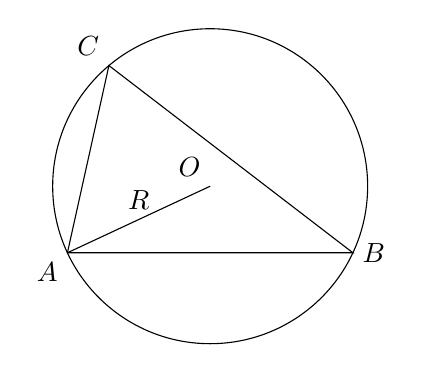
\begin{tikzpicture}
        \coordinate (O) at (0,0);
        \coordinate (B) at (-25:2cm);
        \coordinate (A) at (205:2cm);
        \coordinate (C) at (130:2cm);
        \coordinate (D) at (-90:2cm);
        
        \draw (O) circle (2cm);
        \draw (A) -- (B) -- (C) -- cycle;
        \node[right] at (B) {$B$};
        \node[below left] at (A) {$A$};
        \node[above left] at (C) {$C$};
        \node[above left] at (O) {$O$};
        \draw (A) -- node[above]{$R$} (O);
    \end{tikzpicture}
\end{center}
\subsection{Latihan Soal Teorema Garis Bagi}
\begin{enumerate}
    \item (OSK 2014) Diberikan segitiga $ABC$ dengan $AB = 360, BC = 240,$ dan $AC = 180$. Garis bagi dalam dan garis bagi luar dari $\angle CAB$ memotong $BC$ dan perpanjangan $BC$ berturut-turut di $P$ dan $Q$. Jari-jari lingkaran yang melalui titik-titik $A, P,$ dan $Q$ adalah \dots
    
    \item (OSK 2015) Pada segitiga $ABC$, garis tinggi $AD$, garis bagi $BE$ dan garis berat $CF$ berpotongan di satu titik. Jika panjang $AB = 4$ dan $BC = 5$, dan $CD = \frac{m^2}{n^2}$ dengan $m$ dan $n$ relatif prima, maka nilai dari $m - n$ adalah \ldots
\end{enumerate}
\subsection{Dalil Sinus dan Dalil Cosinus}
    Misalkan $ABC$ adalah suatu segitiga dengan $R$ adalah panjang jari-jari lingkaran luarnya.
\begin{center}
    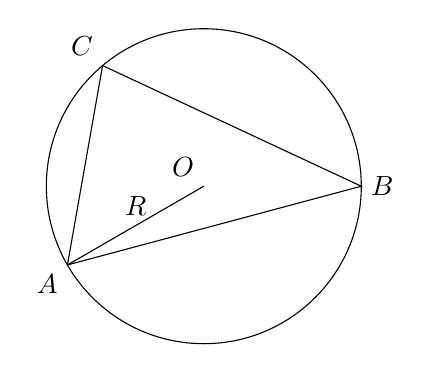
\begin{tikzpicture}
    \coordinate (O) at (0,0);
    \coordinate (B) at (0:2cm);
    \coordinate (A) at (210:2cm);
    \coordinate (C) at (130:2cm);
    
    \draw (O) circle (2cm);
    \draw (A) -- (B) -- (C) -- cycle;
    \node[right] at (B) {$B$};
    \node[below left] at (A) {$A$};
    \node[above left] at (C) {$C$};
    \node[above left] at (O) {$O$};
    \draw (A) -- node[above]{$R$} (O);
    \end{tikzpicture}
\end{center}
    \subsubsection{Dalil Sinus}
    $$\dfrac{BC}{\sin \angle A} = \dfrac{CA}{\sin \angle B}= \dfrac{AB}{\sin \angle C} = 2R$$
    
    \subsubsection{Dalil Cosinus}
    \begin{align*}
        AB^2 &= BC^2 + CA^2 - 2\cdot BC \cdot CA \cdot \cos \angle C\\
        BC^2 &= CA^2 + AB^2 - 2\cdot CA \cdot AB \cdot \cos \angle A\\
        CA^2 &= AB^2 + BC^2 - 2\cdot AB \cdot BC \cdot \cos \angle B
    \end{align*}
\subsection{Latihan Soal Dalil Sinus dan Cosinus}
\begin{enumerate}
    \item (OSK 2016) Pada segitiga $ABC$, titik $M$ terletak pada $BC$ sehingga $AB=7, AM=3, BM=5$, dan $MC=6$. Panjang $AC$ adalah \dots

    \item (OSK 2013) Misalkan $P$ adalah titik interior dalam daerah segitiga $ABC$ sehingga besar $\angle PAB = 10^\circ, \angle PBA = 20^\circ, \angle PCA = 30^\circ, \angle PAC=40^\circ$. Besar $\angle ABC = \dots$
    
    \item (LMNAS SMP 33 Penyisihan) Diberikan segitiga tumpul $ABC$ dengan $AB = BC$. Titik $D$ berada di dalam segitiga tersebut sedemikian sehingga $AD = BD$, $\angle ADB = 140^\circ$, dan $\angle ADC = 150^\circ$. Besar sudut $ACD$ dalam satuan $^\circ$ (derajat) adalah \dots
    
    \item (Modifikasi OSK 2017) Pada sebuah lingkaran dengan pusat $O$, talibusur $AB$ berjarak 5 dari titik $O$ dan talibusur $AC$ berjarak $5\sqrt{2}$ dari titik $O$ dengan titik $A$ terletak di busur $BC$ yang lebih kecil ($A$ diantara $B$ dan $C$) Jika panjang jari-jari lingkaran 10, maka $BC^2=\dots$
\end{enumerate}
\subsection{Dalil Stewart}
    Pada segitiga $ABC$ dengan titik $D$ pada segmen $BC$, dimana $AB=c, BC=a, CA=b, AD=d, BD=m, CD=n$, maka berlaku
    \begin{align*}
        BC \cdot AD^2 + BC \cdot BD \cdot CD &= CA^2 \cdot BD + AB^2 \cdot CD\\
        ad^2+amn &= b^2m+c^2n
    \end{align*}
\begin{center}
    \begin{tikzpicture}
    % titik-titik segitiga
    \coordinate[label=left:$C$]  (C) at (-1.5cm,-1.cm);
    \coordinate[label=right:$B$] (B) at (1.5cm,-1.0cm);
    \coordinate[label=above:$A$] (A) at (0.5cm,1.732cm);
    % titik-titik cevian
    \coordinate[label=below:$D$] (D) at ($(C)!0.3!(B)$);
    
    % pembuatan segitiga
    \draw (A) -- node[right]{$c$} (B) -- node[above]{$m$} (D) -- node[above]{$n$} (C) -- node[left]{$b$} (A);
    
    
    % pembuatan cevian
    \draw (B) --node[below]{$a$}(C);
    \draw (A) --node[right]{$d$}(D);
    \end{tikzpicture}
\end{center}
\subsection{Latihan Soal Dalil Stewart}
\begin{enumerate}
    \item (OSK 2016) Pada segitiga $ABC$, titik $M$ terletak pada $BC$ sehingga $AB=7, AM=3, BM=5$, dan $MC=6$. Panjang $AC$ adalah \dots

    \item (HMMT 1999) Dalam segitiga $ABD$, $F$ berada pada segmen $AD$, $E$ berada pada sinar $BF$, $G$ berada pada segmen $BD$, dan $C$ adalah titik perpotongan dari $FG$ dan $ED$. Diketahui bahwa $AB = 15$, $BD = 18$, $AF = 15$, $DF = 12$, $BE = 24$, dan $CF = 17$. Temukan rasio $BG : FG$.
    % https://drive.google.com/drive/search?q=parent:0B-4OltLGFEDFeG92VENBbmdZODA%20type:pdf%20menelaus
\end{enumerate}
\subsection{Dalil Ceva}
Jika pada segitiga $ABC$, titik $D,E,F$ berturut-turut berada di segmen $BC$,$CA$,$AB$, maka 
$AD,BE,CF$ konkuren atau berpotongan di satu titik jika dan hanya jika $$\dfrac{AF}{FB} \cdot \dfrac{BD}{DC} \cdot \dfrac{CE}{EA} = 1.$$
\begin{center}
    \begin{tikzpicture}
    % titik-titik segitiga
    \coordinate[label=left:$A$]  (A) at (-1.5cm,-1.cm);
    \coordinate[label=right:$B$] (B) at (1.5cm,-1.0cm);
    \coordinate[label=above:$C$] (C) at (0.5cm,1.732cm);
    
    % pembuatan segitiga
    \draw (A) -- (B) -- (C) -- cycle;
    
    % titik-titik cevian
    \coordinate[label=below:$F$] (F) at ($(A)!0.7!(B)$);
    \coordinate[label=right:$D$] (D) at ($(B)!0.5!(C)$);
    \coordinate[label=left:$E$]  (E) at ($(C)!0.3!(A)$);
    
    % pembuatan cevian
    \draw (A) -- (D);
    \draw (B) -- (E);
    \draw (C) -- (F);
    \end{tikzpicture}
\end{center}
\subsection{Latihan Soal Dalil Ceva}
\begin{enumerate}
    \item (OSK 2015) Pada segitiga $ABC$, garis tinggi $AD$, garis bagi $BE$ dan garis berat $CF$ berpotongan di satu titik. Jika panjang $AB = 4$ dan $BC = 5$, dan $CD = \frac{m^2}{n^2}$ dengan $m$ dan $n$ relatif prima, maka nilai dari $m - n$ adalah \ldots
\end{enumerate}

\subsection{Dalil Menelaus}
Jika pada segitiga $ABC$, titik $P,Q,R$ berturut-turut berada pada garis (bisa di perpanjangan segmen) $BC$,$CA$, $AB$, maka $P,Q,R$ segaris jika dan hanya jika
$$\dfrac{AR}{RB} \cdot \dfrac{BP}{PC} \cdot \dfrac{CQ}{QA} = 1.$$
\begin{center}
    \begin{asy}
        unitsize(10);
        defaultpen(fontsize(8));
        pair P=(7,6), Q=(0,0), C=(10,0), A=(4,0), B=(6,8), R;
        draw((A)--(B)--(C)--cycle,blue+0.75);
        draw(P--R--Q--A);
        R=intersectionpoint(A--B,Q--P);
        dot(A^^B^^C^^P^^Q^^R);
        label("A",A,(0,-1));label("B",B,(1,0));label("C",C,(1,0));label("P",P,(1,1));label("Q",Q,(-1,0));label("R",R,(-1,1));
    \end{asy}
\end{center}
\subsection{Latihan Soal Dalil Menelaus}
\begin{enumerate}
    \item Dalam segitiga $ABD$, $F$ berada pada segmen $AD$, $E$ berada pada sinar $BF$, $G$ berada pada segmen $BD$, dan $C$ adalah titik perpotongan dari $FG$ dan $ED$. Diketahui bahwa $AB = 15$, $BD = 18$, $AF = 15$, $DF = 12$, $BE = 24$, dan $CF = 17$. Temukan rasio $BG : FG$.
    % https://drive.google.com/drive/search?q=parent:0B-4OltLGFEDFeG92VENBbmdZODA%20type:pdf%20menelaus

    \item (OSK 2022) Diberikan $ABC$ siku-siku sama kaki dengan $BC=AB$. Misalkan $L$ titik tengah $BC$ dan $P$ pada sisi $AC$ sehingga $BP \perp AL$. Jika $CP=30\sqrt{2}$, maka panjang $AB$ adalah \ldots

    \item Diberikan segitiga $ABC$ dengan panjang $BC = 36$. Misalkan $D$ adalah titik tengah $BC$ dan $E$ adalah titik tengah $AD$. Misalkan pula bahwa $F$ adalah perpotongan $BE$ dengan $AC$. Jika diketahui bahwa $AB$ menyinggung lingkaran luar segitiga $BFC$, hitunglah panjang $BF$.
\end{enumerate}
\subsection{Dalil Ptolemy}
    Diketahui sebuah segiempat siklis $ABCD$ maka berlaku
    $$AB \cdot CD + BC \cdot DA = AC \cdot BD.$$

\begin{center}
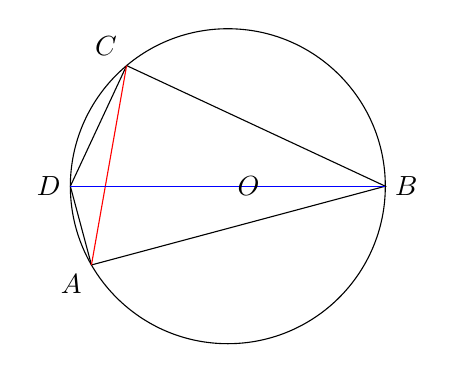
\begin{tikzpicture}
\coordinate (O) at (0,0);
\coordinate (B) at (0:2cm);
\coordinate (A) at (210:2cm);
\coordinate (D) at (180:2cm);
\coordinate (C) at (130:2cm);

\draw (O) circle (2cm);

\draw (A) -- (B) -- (C) -- (D) -- cycle;
\draw[red] (A) -- (C);
\draw[blue] (B) -- (D);

\node[right] at (B) {$B$};
\node[below left] at (A) {$A$};
\node[left] at (D) {$D$};
\node[above left] at (C) {$C$};
\node[right] at (O) {$O$};
\end{tikzpicture}
\end{center}
\subsection{Latihan Soal Dalil Ptolemy}
\begin{enumerate}
    \item Diberikan sebuah segiempat siklis $ABCD$ dengan $ABC$ adalah segitiga sama sisi. Jika $AD=2$ dan $CD=3$, panjang $BD=\dots$
\end{enumerate}